\documentclass{article}
\usepackage[utf8]{inputenc}
\usepackage{textcomp}
\usepackage{booktabs,rotating,tabularx}
\usepackage{graphicx}
\usepackage{xcolor}
\usepackage[english]{babel}
\usepackage{caption}
\usepackage{float}
\usepackage{hyperref} % provides \url{}
\usepackage[shortlabels]{enumitem} % enumeration package
\usepackage[position=top]{subfig} % to use subfloats (used for mockups)
\usepackage{pdfpages}
\usepackage{listings}
\usepackage{tabularx}
\usepackage{float}
\floatplacement{table}{h}


% page layout and margin
\usepackage[a4paper, margin=2.54cm]{geometry}

% list spacing
\usepackage{enumitem}
\setlist{topsep=2pt, itemsep=2pt, partopsep=2pt, parsep=2pt}
\def\arraystretch{2}
% Header & Footer
\usepackage{fancyhdr}
\pagestyle{fancy}
\lhead{Software Engineering 2 - RASD}

\newcommand{\usecase}[9]{
    \def\arraystretch{1.5} % This adds padding to table rows (and more)
    \subsubsection*{Use case [U#2]: #3}
    \vspace*{0.2cm}
    \begin{center}
     \begin{tabular}{|l|p{12cm}|}
         \hline
         \textbf{Actor(s)} & #4 \\
         \hline
         \textbf{Entry Condition} & #5 \\
         \hline
         \textbf{Event Flow} & #6 \\
         \hline
         \textbf{Exit Condition} & #7 \\
         \hline
          \textbf{Exceptions} & #8 \\
         \hline
         \textbf{Notes} & #9 \\
         \hline
      \end{tabular}
    \end{center}
    #1
}

\begin{document}

% title section
\begin{titlepage}
  \centering
  {\normalsize
    Software Engineering 2 - Prof. Matteo Camilli \\
    Dipartimento di Elettronica, Informazione e Bioingegneria \\
    Politecnico di Milano \par
  }     \vspace{3cm}
  {\Huge \textbf{CKB - CodeKataBattle\\} } \vspace{1cm}
  {\large \textbf{RASD\\Requirement Analysis and Specification Document} \par} \vspace{1cm}
  {\normalsize December 22, 2023 \par} \vspace{4cm}
  {\normalsize Emanuele Pocelli (10726303) \\ Fabrizio Sordetti (10730069) \\  Andrea Varesi (10724377)\par} \vspace{4cm}
  \begin{figure}[h]
    \centering
    
\includegraphics[scale=0.3]{src/poli_logo.png}
  \end{figure} \vspace{0.5cm}
\end{titlepage}


\begin{large}

\tableofcontents


\section{Introduction}

\vspace{24pt}

\subsection{Purpose}
The system has, as main function, to deliver a platform where Students can challenge themselves, alone or in team, writing code to solve exercises assigned by Educators, to improve their software development skills. Students have to follow a test-first approach.
\\The platform is used by Educators to create, manage and close tournaments, each one is composed by battles, while Students have to solve the exercises published for every battle filling them with their own code. Each exercise includes a brief textual description and a software project with build automation scripts that contains a set of test cases that the program must pass, but without the program implementation.
\\CKB offres also the possibility for each team to know their rank (calculated automatically by the platform) within the context of each battle, and the general rank of that tournament, in addition to a set of badges the Students can achieve, to increase the level of challenge. 

\vspace{24pt}

\subsubsection{Goals}
$[G1]$ Educator can manage (create battles and badges, grant permission to other Educators, and close) each tournament he/she creates. 
\\$[G2]$ Educator can manage (deliver exercise, set options, evaluate teams submissions and check rank) each battle he/she creates.
\\$[G3]$ Student can subscribe to a tournament.
\\$[G4]$ Student can manage (subscribe and check rank) their participation to a battle.
\\$[G5]$ Both educators and students can check rank for each tournament.
\\$[G6]$ Both educators and students can visualize the profile of a Student.
\\$[G7]$ Both educators and students can see the list of ongoing tournaments.


\newpage

\subsection{Scope}
In recent years, it has gained more and more ground the possibility to train and improve writing code skills through platforms, such as CodeKataBattle, that assign to people who want to challenge themselves exercises to fulfill autonomously, in a programming language of choice. 
\\The philosophy behind these platforms is called \textit{codekata}, a method that aims to refine people's software development skills training and solving excercises over and over again, using feedback to get better every time.
\\CodeKataBattle deals with two main users on its platform:
\begin{itemize}
    \item Educators
    \item Students
\end{itemize}
Each Educator can create a tournament, either creating battles by him/herself or granting to other Educators the permission to create battles within the context of a specific tournament.
\\Once a new tournament is created, all the Students subscribed to CKB are notified and can decide whether to subscribe to that tournament or not. If a Student decides to subscribe to a tournament, he/she will be notified whenever a new battle is created in the context of that tournament. 
\\An Educator that has the permission to do it can create a new battle, and delivers the exercise associated to it. Moreover, the Educator can set the rules for that specific battle.
\\If a Student subscribes to a specific battle, he/she is asked to build his/her own team, with reference to the limits imposed by the Educator. When the deadline expires, for each team is created a GitHub repository, and each team is asked to modify settings, so that for every push the team does, CKB is notified.
\\If the platform is triggered, it pulls the leatest sources of the team from which it has received the notification and automatically evaluates it. Then, it updates the team rank in the context of the battle.
\\When the submission deadline expires, there is an intermediate phase, called consolidation stage, in which Educators manually evaluate team projects, if it is required by the battle's settings.
\\After that, the students partecipating to that battle are notified by the platform and they can visualize their final rank, as well as thier tournament rank, which is updated by CKB whenever a battle ends in the context of that specific torunament.  
\\In every tournament, Students can achieve some Badges, defined by Educators when they create a new tournament.
\\Every user subscribed to the platform can visualize the list of ongoing tournaments, the corresponding tournament rank and other Student's profile, including the badges achieved.

\vspace{24pt}

\subsubsection{World Phenomena}
$[WP1]$ Students work on the assigned exercise.
\\$[WP2]$ Students fork the GitHub repository of the code kata and set up an automated workflow that informs the CKB platform as soon as students push a new commit into the main branch of their repository.

\vspace{12pt}

\subsubsection{Shared Phenomena - controlled by the World}
$[SP1]$ Educator creates a new tournament.
\\$[SP2]$ Educator creates a new battle.
\\$[SP3]$ Educator grants another Educator the permission to create battles within the context of a specific tournament.
\\$[SP4]$ Educator delivers the exercise for a specific battle.
\\$[SP5]$ Educator sets the minimum and maximum number of students per group for a specific battle.
\\$[SP6]$ Educator sets the registration deadline for a specific battle.
\\$[SP7]$ Educator sets the final submission deadline for a specific battle.
\\$[SP8]$ Educator eventually sets the possibility of manually evaluating the projects for a specific battle.
\\$[SP9]$ Student can subscribe to a tournament.
\\$[SP10]$ Student can subscribe to a battle.
\\$[SP11]$ Student can form a team for a specific battle.
\\$[SP12]$ Both students and educators involved in the battle can see the current rank evolving during the battle.
\\$[SP13]$ Educator manually evaluates the projects for a specific battle (consolidation stage).
\\$[SP14]$ Both Educators and Students subscribed to CKB can see the list of ongoing tournaments as well as the corresponding tournament rank.
\\$[SP15]$ Educator can define a Badge for a specific tournament.
\\$[SP16]$ Both Educators and Students can visualize another Student's profile.

\vspace{12pt}
 
\subsubsection{Shared Phenomena - controlled by the Machine}
$[SP17]$ CKB sends a notification to all Students subscribed to the platform whenever a new tournament is created. 
\\$[SP18]$ CKB sends a notification to all Students subscribed to a specific tournament whenever a new battle is created in the context of that specific tournament.
\\$[SP19]$ At the end of the consolidation stage, all students participating in the battle are notified when the final battle rank becomes available.
\\$[SP20]$ When an educator closes a tournament, as soon as the final tournament rank becomes available, the CKB platform notifies all students subscribed to that tournament.
\\$[SP21]$ CKB can assign a Badge to a Student.

\vspace{24pt}

\newpage

\subsection{Definitions, Acronyms, Abbreviations}

\vspace{24pt}

\subsubsection{Definitions}
\begin{itemize}
    \item \textbf{Programming language}: set of rules that allows string values to be converted into various ways of generating machine code, or, in the case of visual programming languages, graphical elements.
    \item \textbf{Automation scripts}: a specific type of automation script used in software development to automate the process of building, compiling, and packaging software applications.
    \item \textbf{Test-first approach}: is a software development process relying on software requirements being converted to test cases before software is fully developed, and tracking all software development by repeatedly testing the software against all test cases.
    \item \textbf{GitHub}: a platform and cloud-based service for software development and version control, allowing developers to store and manage their code.
    \item \textbf{Badge}: elements in the form of rewards that represent the achievements of individual students.
\end{itemize}

\vspace{12pt}

\subsubsection{Acronyms}
\begin{itemize}
    \item \textbf{CKB}: CodeKataBattle
    \item \textbf{RASD}: Requirement Analysis and Specification Document
    \item \textbf{UML}: Unified Modelling Language
    \item \textbf{UI}: User Interface
    \item \textbf{OWASP}: Open Web Application Security Project
    \item \textbf{WCAG}: Web Content Accessibility Guidelines
\end{itemize}

\vspace{12pt}

\subsubsection{Abbreviations}
\begin{itemize}
    \item $[Gn]$ - the n-th goal of the system
    \item $[WPn]$ - the n-th world phenomena
    \item $[SPn]$ - the n-th shared phenomena
    \item $[UCn]$ - the n-th use case
    \item $[Rn]$ - the n-th functional requirement
\end{itemize}

\vspace{24pt}

\subsection{Revision history}
\begin{itemize}
    \item Version 1.0 (22/12/2023);
\end{itemize}

\vspace{24pt}

\subsection{Reference Documents}

This document is based on: 
\begin{itemize}
    \item The specification of the RASD and DD assignment of the Software Engineering II course, held by professor Matteo Rossi, Elisabetta Di Nitto and Matteo Camilli at the Politecnico di Milano, A.Y 2023/2024
    \item Slides of Software Engineering 2 course on WeBeep;
    \item Official link of Codewars (https://www.codewars.com/), a platform similar to CodeKataBattle
    \item Other informations that helped the development of the project: 
    \begin{itemize}
        \item In-depth analysis on \href{http://codekata.com/}{codekata};
        \item In-depth analysis on \href{https://en.wikipedia.org/wiki/Test-driven\textunderscore development}{test-driven development};
    \end{itemize}
\end{itemize}

\vspace{24pt}

\subsection{Document Structure}

This document is divided in 6 chapters, more in detail:
\begin{enumerate}
    \item \textbf{Introduction}: this chapter describes the reasons for which this project is being developed, highlighting above all the goals aimed to reach. Moreover, it analyses the environment and the shared phenomena between the world and the machine.
    \item \textbf{Overall description}: it is an initial analysis about the system to be developed, with examples of possible scenarios. In particular it focuses, through diagrams (e.g. class diagrams, state diagrams), on the elements in the system's domain and the interaction between them. This section also includes domain assumptions and the most relevant requirements of the system.
    \item \textbf{Specific requirements}: this chapter aims to describe all the system's requirements, both functional and non-functional, and eventual constraints. Diagrams are used to integrate requirements with scenarios and generalize them into use cases. 
    \item \textbf{Formal analysis using Alloy}: this chapter describes, with Alloy language, the entire model in a formal way. There is also an overview about what can be verified and some examples of the world obtained running the code.
    \item \textbf{Effort spent}: this section shows the time spent (in hours) by each member to work on this document.
    \item \textbf{References}: it contains the references to any documents and to the Software used in this document.
\end{enumerate}

\definecolor{myred}{rgb}{0.99, 0.0, 0.0}
\section{Overall Description}

\subsection{Product perspective}
\subsubsection{Scenarios}
\begin{enumerate}[label=\textbf{\Alph*}.]
    \item \textbf{Registration} \\
        Emanuele is a Computer Science and Engineering student. He wants to showcase and develop his programming skills. He heard about CKB and decides to give it a try. He goes to the CKB website and creates an account providing his personal info, his academic status (student/educator),  and setting up a password. After that, he can join tournaments and finally start showing off his abilities while becoming a code master in the process.\\
    \item \textbf{Tournament creation} \\
        Matteo is a Google hiring manager. He is looking for new talented and enthusiastic software engineers. He creates a new tournament specifying the deadline for the subscription and grants his team permission to create new battles. Users who enabled notifications will receive an email notifying them about the creation of this new tournament. Matteo finds a lot of passionate coders and engages with them in a wide variety of battles. He can then pick those who performed brilliantly and can offer them a job at Google.\\
    \item \textbf{Battle creation} \\
        Giuseppe is a recruiter from Google with an 'educator' account in CKB. He has been granted permission to create battles  by his superior, Matteo. He publishes the code kata (that includes everything to make the battle work, from the description to test cases and automation scripts) and chooses edits the battle configuration settings such as minimum and maximum number of students per team, submission deadline and more. Students subscribed to this tournament can form teams and start working on the project. After the submission deadline, teams will receive an automatic evaluation. Giuseppe is allowed to review the evaluations if need be, and finally publish the final grades for each team.  \\ 
    \item \textbf{Badge creation} \\
        Matteo wants to add achievements to his tournament to hype up the students. He chooses a few conditions that he finds interesting selects the titles and creates the badges. At the end of the tournament, all the system checks the badges conditions to each user. Ultimately, the badges will be assigned to the students and they will be able to show them in their personal profile.
\end{enumerate}

\subsubsection{Class diagram}
The presented UML class diagram illustrates a conceptual, high-level model of the software. Due to its nature, it might model entities that won't necessarily be part of the final system under development. At this stage, it lacks references to methods and other low-level details, as these will be elaborated during the subsequent design phase.
\begin{figure}[H]
      \centering
      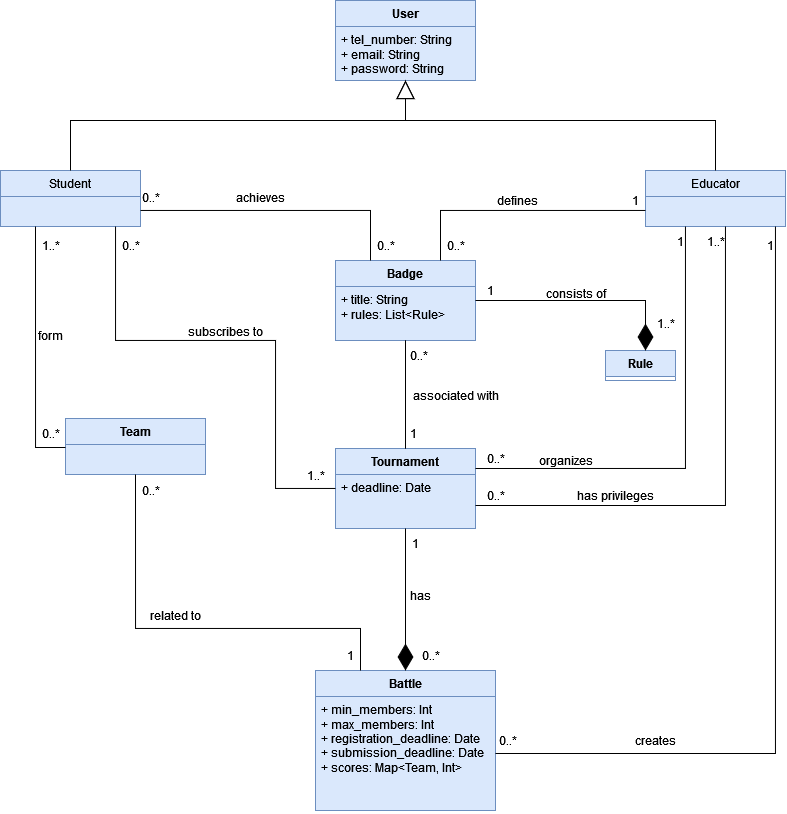
\includegraphics[scale=0.4]{src/class_uml.png}
\end{figure} \vspace{1cm}

The main entities are:
\begin{itemize}
    \item \textbf{User}\\
        A user can be either a student or an educator. Users can perform different actions according to this: educators create tournaments and battles, while students join them.
    \item \textbf{Tournament}\\
        Tournaments are created by educators and students can subscribe to them. They consist of different battles. The creator of the tournament can grant other educators privileges to define battles. Each student has a score consisting of the cumulative sum of scores obtained in all battless. Badges can also be assigned to a specific tournament.
    \item \textbf{Battles}\\
        Battles are created by educators with privileges in the scope of a tournament. Numerous settings are available for customization, such as the minimum and maximum settings for a team, deadlines and more. Students subscribed to a tournament need to form a team for each battle. At the end of the battle, each team is assigned a score between 0 and 100.
    \item \textbf{Badge}\\
        Badges are gamification objects that students can collect and show off in their profile. Educators can create badges and associate them to a specific tournament. Each badge has a set of rules that students need to satisfy in order to achieve It.
\end{itemize}

\subsubsection{State diagrams}
The purpose of the following UML state diagrams is to provide additional information about the behaviour of the system. These are the scenarios that we found more interesting.

\begin{figure}[H]
      \centering
      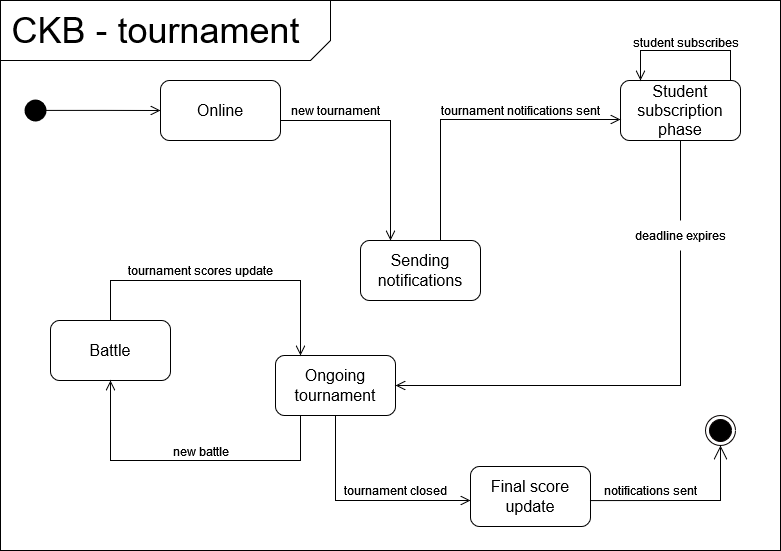
\includegraphics[scale=0.4]{src/state_diagrams/tournament_uml.png}
      \caption{Tournament timeline}
\end{figure} \vspace{1cm}
    This diagram describes what happens inside the system throughout a tournament, from the creation to the conclusion. At first, the system is waiting for new events. When an educator creates a new tournament, the system responds by sending notifications to all students. After that, the system enters a waiting state, allowing students to subscribe to the tournament until the specified deadline. When the tournament is finally open, authorized educators can create new battles. This process is seen more in-depth in the next diagram. After each battle, the system automatically updates the score for each student. New battles can be created until the creator closes the tournament. Students who took part in this tournament are sent a notification about their score, their ranking and eventual badges they may have achieved. At any moment, the creator can grant other educators permission to create battles in the scope of his tournament.\\

\begin{figure}[H]
      \centering
      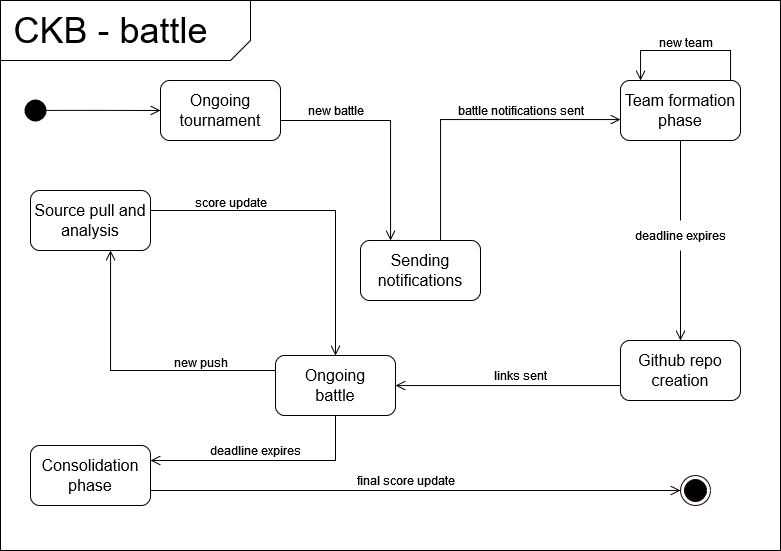
\includegraphics[scale=0.4]{src/state_diagrams/battle_uml.png}
      \caption{Battle timeline}
\end{figure} \vspace{1cm}
    This diagrams describes the steps of a battle. When a new battle is created in the scope of a tournament, the system sends a notification to all students subscribed to that tournament. Students have some time to form teams and after the deadline, a github repository is automatically created. Teams can then start working on the project. The system is notified through API calls every time a team pushes new code. Following each push, the system downloads and evaluates the sources, then publishes the scores up to that point. The specifics of these calls are beyond the scope of this diagram. After the deadline, there is a consolidation phase, where authorized educators can manually adjust the scores if need be. Finally, the battle officially ends and the students are notified.

\subsection{Product Functions}
\subsubsection{User Registration and Authentication}
\begin{itemize}
    \item \textbf{User Registration}: Users can create accounts on the CKB platform by providing necessary information such as academic position (educator or student), email address and password. The registration process includes validation and email verification.
    \item \textbf{Authentication}: Once registered, users can log in with their credentials to access the platform. Authentication ensures that only authorized users can use the platform and the available functions are restricted depending on the user.
    \item \textbf{User Account Management}: Registered users have the ability to manage their account settings, update their profile information, and change passwords as needed.
\end{itemize}

\subsubsection{Creating and Managing Tournaments}
\begin{itemize}
    \item \textbf{Tournament Creation}: Educators, who act as administrators, can create new tournaments. They provide details about the tournament, including its name, description, duration, and any specific rules.
    \item \textbf{Tournament Management}: Educators can modify and manage existing tournaments. They can update tournament details, add or remove battles, and set deadlines for registration and submission. They can add other Educators to administer the tournament, too.
\end{itemize}

\subsubsection{Joining and Forming Teams}
\begin{itemize}
    \item \textbf{Joining Battles}: Students can browse and subscribe to available tournaments and join specific battles within those tournaments. They can view information about battles, such as the code kata description and participation rules.
    \item \textbf{Team Formation}: Students can form teams by inviting other students to join them. The system checks that they adhere to the minimum and maximum team size rules set by the educator.
\end{itemize}

\subsubsection{Code Kata Battles}
\begin{itemize}
    \item \textbf{Accessing Projects}: Students participating in a battle can download the respective project. Each project consists of a problem description and an initial codebase with missing functionality.
\end{itemize}
\subsubsection{GitHub Integration}
\begin{itemize}
    \item \textbf{GitHub Repository Creation}: For each code kata, the platform creates a corresponding GitHub repository for each team. This repository contains the initial codebase and testing scripts.
    \item \textbf{Updating and Testing Projects}: Students set up GitHub Actions to automate the submission process. With each code commit to their repository, GitHub Actions trigger updates and testing on the platform.
\end{itemize}
\subsubsection{Scoring and Ranking}
\begin{itemize}
    \item \textbf{Score Calculation}: The platform calculates scores based on the number of passed test cases, timeliness of submissions, and code quality. The higher the number of passing test cases, the higher the score.
    \item \textbf{Ranking System}: Students can view the real-time ranking of their teams and others in the same battle. Rankings are based on scores achieved during the competition.
\end{itemize}

\subsubsection{Consolidation and Manual Evaluation}
\begin{itemize}
    \item \textbf{Consolidation Stage}: After the submission deadline, educators review the code and manually evaluate aspects that cannot be determined automatically, such as code quality and innovation.
    \item \textbf{Final Ranking}: Once the consolidation stage is complete, the final ranking is determined, and students are notified of their positions and scores.
\end{itemize}
\subsubsection{Gamification and Badges}
\begin{itemize}
    \item \textbf{Badge Definition}: Educators can create gamification badges with specific titles and rules. 
    \item \textbf{Badge Assignment}: The badges are awarded to students based on the rules defined by the educators.
\end{itemize}
\subsubsection{Notification and Communication}
\begin{itemize}
    \item \textbf{Notification System}: The platform sends notifications to students about various events, such as new tournament announcements, battle updates, and final tournament rank confirmations.
\end{itemize}

\subsubsection{Profile and Tournament Statistics}
\begin{itemize}
    \item \textbf{User Profiles}: Each user has a profile that displays their personal information, tournament participation, and badges earned.
    \item \textbf{Tournament Statistics}: Users can view statistics related to their performance in each tournament, including scores, rankings, and tournament history.
\end{itemize}

\subsection{User characteristics}
There are mainly two kinds of users that interact with the system: Educator and Student.
\subsubsection{Educator}
\begin{itemize}
    \item \textbf{Teaching Level}: Educators can be university professors, instructors, or trainers responsible for organizing and supervising code kata battles.
    \item \textbf{Educational Institution}: They may work in educational institutions and have experience in teaching software development.
    \item \textbf{Platform Experience}: Educators should be familiar with the CodeKataBattle platform to create and manage tournaments, set up battles, and assess student performance.
    \item \textbf{Technical Proficiency}: While not all educators need to be technically proficient, some may have a background in software development and programming.
\end{itemize}
\subsubsection{Student}
\begin{itemize}
    \item \textbf{Programming Proficiency}: Students may vary in their level of programming proficiency, ranging from beginners to advanced developers.
    \item \textbf{Educational Level}: Students from various educational backgrounds, such as undergraduate, graduate, or coding boot camp participants, may use the platform.
    \item Motivation: Students may use the platform for different reasons, including academic requirements, self-improvement, or competition.
    \item \textbf{Preferred Programming Languages}: Users may have preferences for specific programming languages and may select code katas accordingly.
    \item \textbf{Team Formation}: Students can either participate individually or form teams based on the requirements of specific battles.
    \item \textbf{Time Availability}: Students have different schedules and availability for participating in code kata battles.
\end{itemize}
\subsection{Assumptions, dependencies and constraints}
\subsubsection{Regulatory policies}
\begin{enumerate}
    \item \textbf{\textit{Data Privacy and Protection:}}
    \begin{itemize}
        \item \textbf{General Data Protection Regulation (GDPR)}: The CKB platform will ask for user personal information like name, surname and email address. Email addresses won’t be used for commercial purposes. Personal information will be processed in compliance with the GDPR.
    \end{itemize}
    \item \textbf{\textit{Intellectual Property Rights:}}
    \begin{itemize}
        \item \textbf{Copyright and Licensing}: The platform must respect copyright and licensing regulations when handling code katas, user submissions, and other content. It should encourage users to respect the intellectual property rights of others and provide mechanisms for reporting copyright violations.
        \item \textbf{Plagiarism Prevention}: The platform should have mechanisms in place to detect and prevent plagiarism in code submissions. This includes educating users on proper citation and attribution practices.
    \end{itemize}
\end{enumerate}

\subsubsection{Domain Assumptions}
The following are the assumptions made for the domain. Such assumptions are properties and/or conditions that the system takes for granted, mostly because they are out of the control of the system itself, and hence need to be verified to assure the correct behavior of CKB.
\\$[D1]$: Users have reliable and consistent access to the internet to participate in code kata battles and interact with the platform.
\\$[D2]$: Users have access to suitable devices, such as computers or mobile devices, with compatible web browsers.
\\$[D3]$: Educators have a basic understanding of the CodeKataBattle platform's features, enabling them to create and manage tournaments and battles effectively. In particular, they have to provide correct tests and rules for projects and badges.
\\$[D4]$: User-provided data, including user profiles, code submissions, and scoring information, is assumed to be accurate and valid. Users are supposed to providing truthful information.
\\$[D5]$: Users will use the platform responsibly, adhering to ethical guidelines and academic integrity. Students are expected to complete code katas independently or within the rules of team collaboration defined by educators.
\\$[D6]$: The platform assumes a high level of system uptime, with minimal downtime, to support user interactions, database storage, and real-time features.
\\$[D7]$: Some platform functionalities may rely on external services, such as email verification, communication tools and Github integrations. These external services are assumed to be available and functional.
\\$[D8]$: Users are responsible for maintaining the security and privacy of their accounts, including choosing strong passwords and keeping their login credentials confidential.
\\$[D9]$: Users are expected to engage in ethical behavior, respecting intellectual property rights, academic integrity, and community guidelines established by the platform.
\include{section/Specific_Requirements.tex}
\section{Alloy}

In the following are stated all the signatures defined for the Alloy modelization.
\vspace{0.5 cm}
\lstinputlisting[language=alloy]{src/Alloy-RASD.als}

\vspace{2cm}

\begin{figure}[h]
    \centering
    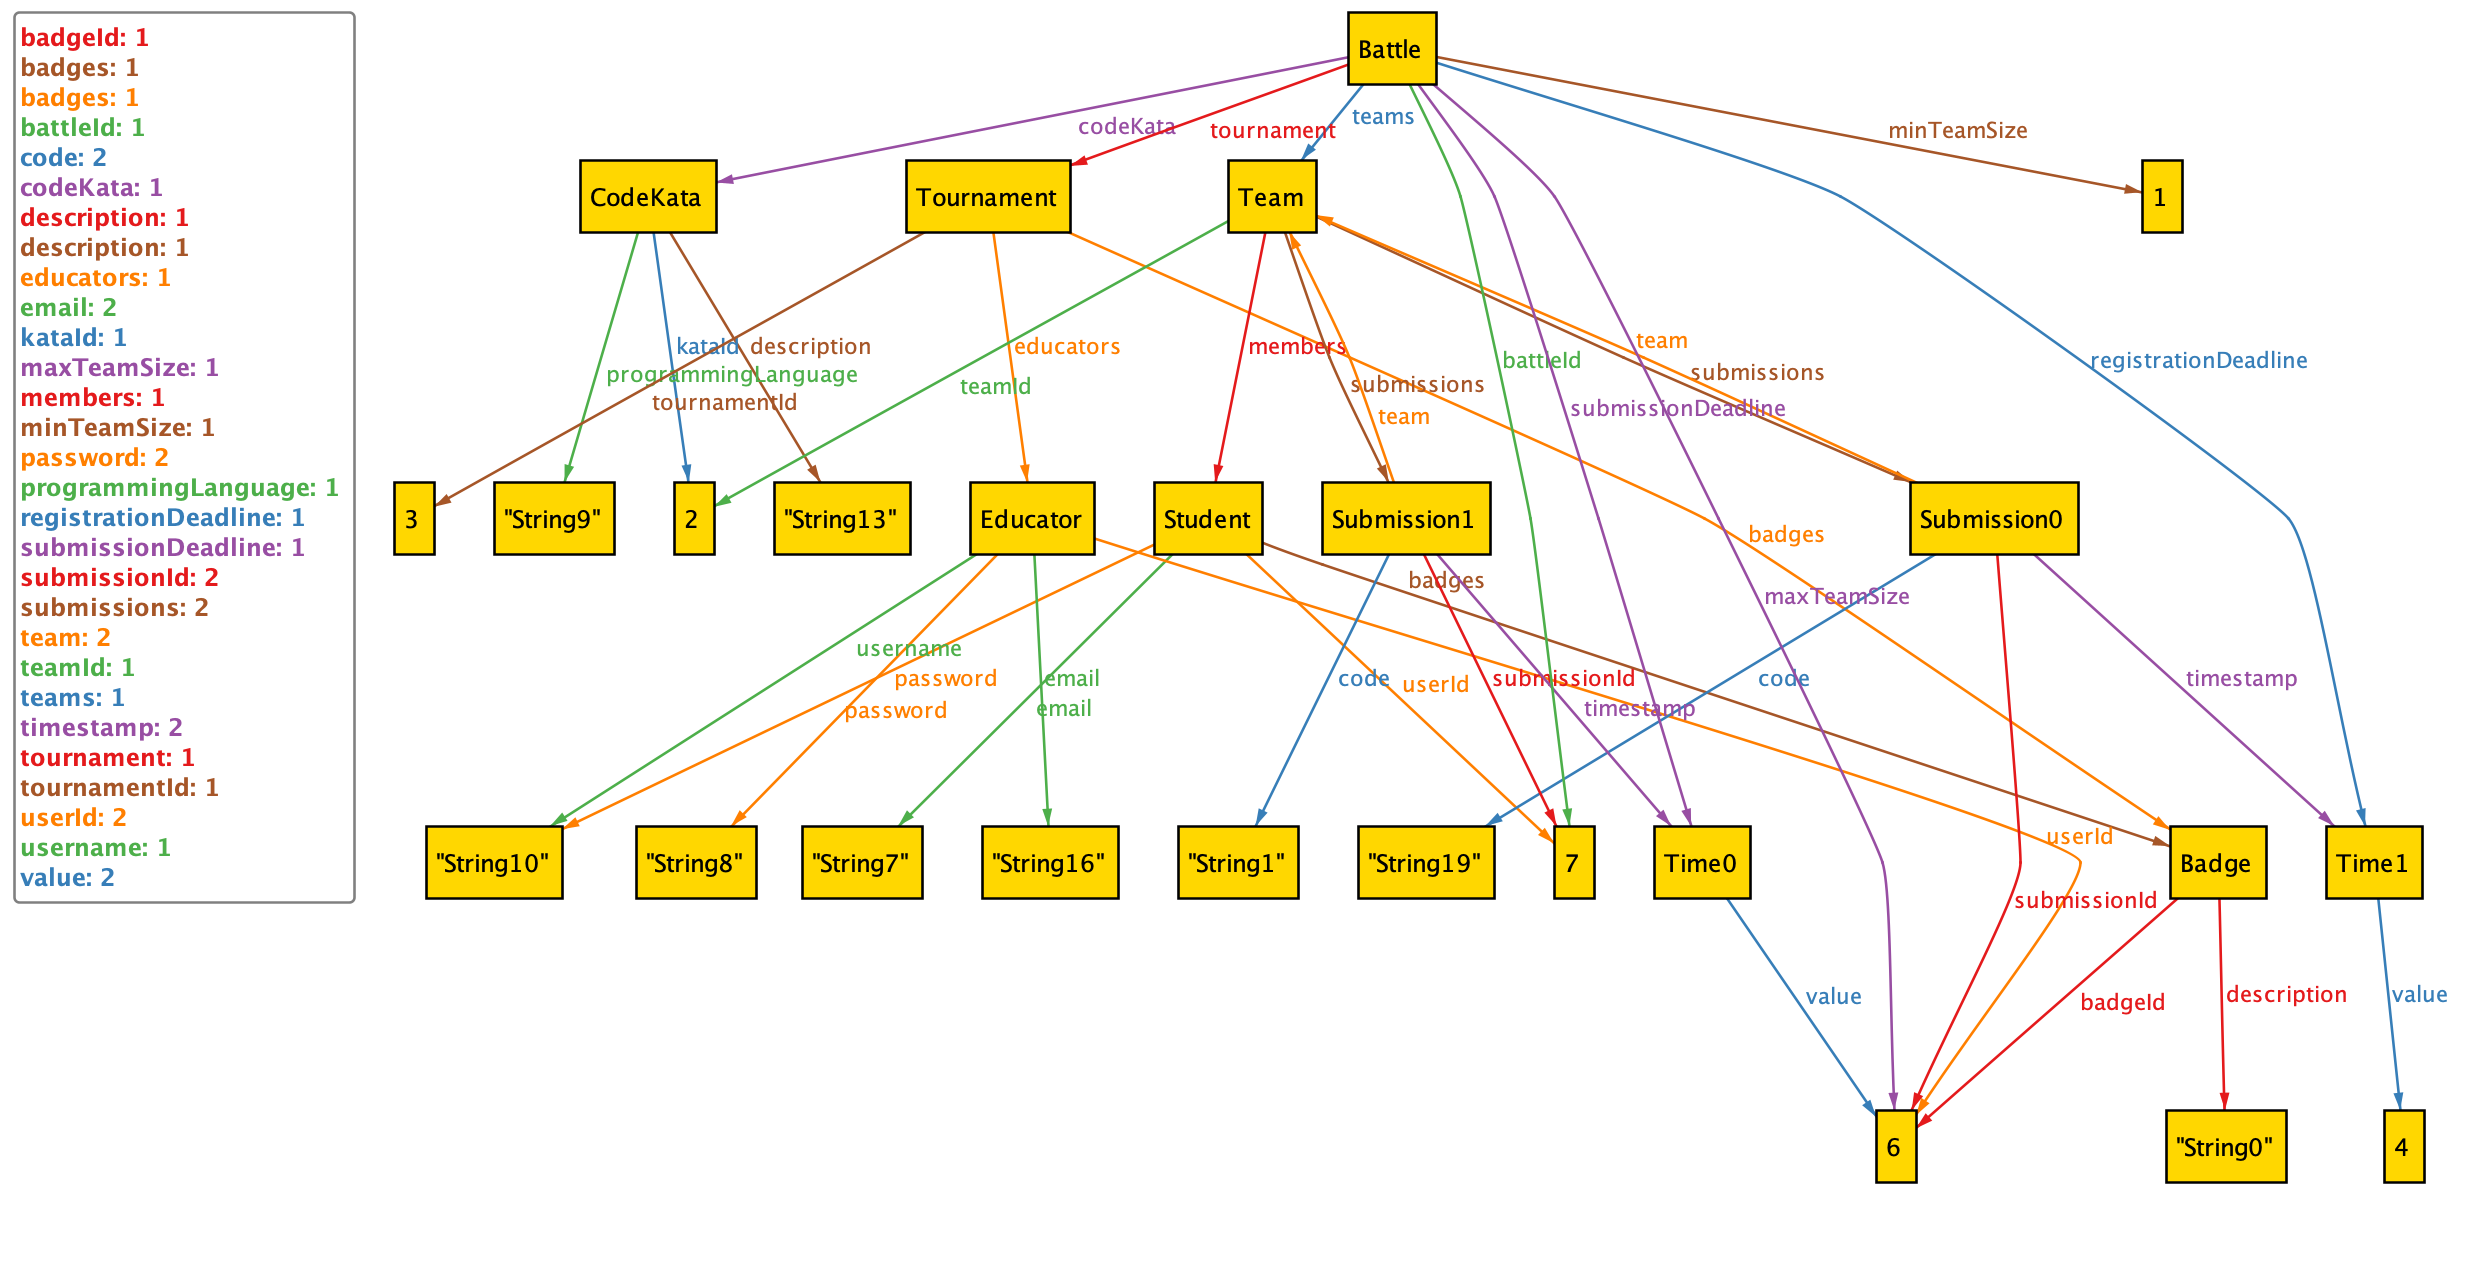
\includegraphics[width=\textwidth]{src/Alloy-model.png}
    \caption*{Alloy Model}
\end{figure} \vspace{0.5cm}

\section{Effort Spent}


\begin{table}[h]
  \centering
  \caption*{Emanuele Pocelli}
  \begin{tabularx}{\textwidth}{|X|X|}
    \hline
    \textbf{Chapter} & \textbf{Effort (in hours)}\\
    \hline
    1 & 1\\
    \hline
    2 & 25\\ 
    \hline
    3 & 2\\
    \hline 
    4 & 2\\ 
    \hline
    5 & 2\\
    \hline
  \end{tabularx}
\end{table}

\begin{table}[h]
  \centering
  \caption*{Fabrizio Sordetti}
  \begin{tabularx}{\textwidth}{|X|X|}
    \hline
    \textbf{Chapter} & \textbf{Effort (in hours)}\\
    \hline
    1 & 1\\
    \hline
    2 & 25\\
    \hline
    3 & 1\\
    \hline 
    4 & 3\\
    \hline
    5 & 3\\
    \hline
  \end{tabularx}
\end{table}

\begin{table}[h]
  \centering
  \caption*{Andrea Varesi}
  \begin{tabularx}{\textwidth}{|X|X|}
    \hline
    \textbf{Chapter} & \textbf{Effort (in hours)}\\
    \hline
    1 & 3\\
    \hline
    2 & 3\\
    \hline
    3 & 5\\
    \hline 
    4 & 6\\
    \hline
    5 & 15\\
    \hline
  \end{tabularx}
\end{table}

\section{References}

\begin{itemize}
    \item Diagrams made with: \href{https://app.diagrams.net}{draw.io}
    \item Mockups made with: \href{https://moqups.com/it/}{moqups.com}
    \item Testing models and component architecture made with: \href{https://app.diagrams.net}{draw.io}
    \item High level architectures are made with: \href{https://app.diagrams.net}{draw.io}
\end{itemize}


\end{large}
\end{document}